% Options for packages loaded elsewhere
% Options for packages loaded elsewhere
\PassOptionsToPackage{unicode}{hyperref}
\PassOptionsToPackage{hyphens}{url}
\PassOptionsToPackage{dvipsnames,svgnames,x11names}{xcolor}
%
\documentclass[
  11pt,
  a4paper,
  DIV=11,
  numbers=noendperiod]{scrartcl}
\usepackage{xcolor}
\usepackage[lmargin=2cm,rmargin=2cm,tmargin=2cm,bmargin=2cm]{geometry}
\usepackage{amsmath,amssymb}
\setcounter{secnumdepth}{-\maxdimen} % remove section numbering
\usepackage{iftex}
\ifPDFTeX
  \usepackage[T1]{fontenc}
  \usepackage[utf8]{inputenc}
  \usepackage{textcomp} % provide euro and other symbols
\else % if luatex or xetex
  \usepackage{unicode-math} % this also loads fontspec
  \defaultfontfeatures{Scale=MatchLowercase}
  \defaultfontfeatures[\rmfamily]{Ligatures=TeX,Scale=1}
\fi
\usepackage{lmodern}
\ifPDFTeX\else
  % xetex/luatex font selection
\fi
% Use upquote if available, for straight quotes in verbatim environments
\IfFileExists{upquote.sty}{\usepackage{upquote}}{}
\IfFileExists{microtype.sty}{% use microtype if available
  \usepackage[]{microtype}
  \UseMicrotypeSet[protrusion]{basicmath} % disable protrusion for tt fonts
}{}
\makeatletter
\@ifundefined{KOMAClassName}{% if non-KOMA class
  \IfFileExists{parskip.sty}{%
    \usepackage{parskip}
  }{% else
    \setlength{\parindent}{0pt}
    \setlength{\parskip}{6pt plus 2pt minus 1pt}}
}{% if KOMA class
  \KOMAoptions{parskip=half}}
\makeatother
% Make \paragraph and \subparagraph free-standing
\makeatletter
\ifx\paragraph\undefined\else
  \let\oldparagraph\paragraph
  \renewcommand{\paragraph}{
    \@ifstar
      \xxxParagraphStar
      \xxxParagraphNoStar
  }
  \newcommand{\xxxParagraphStar}[1]{\oldparagraph*{#1}\mbox{}}
  \newcommand{\xxxParagraphNoStar}[1]{\oldparagraph{#1}\mbox{}}
\fi
\ifx\subparagraph\undefined\else
  \let\oldsubparagraph\subparagraph
  \renewcommand{\subparagraph}{
    \@ifstar
      \xxxSubParagraphStar
      \xxxSubParagraphNoStar
  }
  \newcommand{\xxxSubParagraphStar}[1]{\oldsubparagraph*{#1}\mbox{}}
  \newcommand{\xxxSubParagraphNoStar}[1]{\oldsubparagraph{#1}\mbox{}}
\fi
\makeatother

\usepackage{color}
\usepackage{fancyvrb}
\newcommand{\VerbBar}{|}
\newcommand{\VERB}{\Verb[commandchars=\\\{\}]}
\DefineVerbatimEnvironment{Highlighting}{Verbatim}{commandchars=\\\{\}}
% Add ',fontsize=\small' for more characters per line
\usepackage{framed}
\definecolor{shadecolor}{RGB}{241,243,245}
\newenvironment{Shaded}{\begin{snugshade}}{\end{snugshade}}
\newcommand{\AlertTok}[1]{\textcolor[rgb]{0.68,0.00,0.00}{#1}}
\newcommand{\AnnotationTok}[1]{\textcolor[rgb]{0.37,0.37,0.37}{#1}}
\newcommand{\AttributeTok}[1]{\textcolor[rgb]{0.40,0.45,0.13}{#1}}
\newcommand{\BaseNTok}[1]{\textcolor[rgb]{0.68,0.00,0.00}{#1}}
\newcommand{\BuiltInTok}[1]{\textcolor[rgb]{0.00,0.23,0.31}{#1}}
\newcommand{\CharTok}[1]{\textcolor[rgb]{0.13,0.47,0.30}{#1}}
\newcommand{\CommentTok}[1]{\textcolor[rgb]{0.37,0.37,0.37}{#1}}
\newcommand{\CommentVarTok}[1]{\textcolor[rgb]{0.37,0.37,0.37}{\textit{#1}}}
\newcommand{\ConstantTok}[1]{\textcolor[rgb]{0.56,0.35,0.01}{#1}}
\newcommand{\ControlFlowTok}[1]{\textcolor[rgb]{0.00,0.23,0.31}{\textbf{#1}}}
\newcommand{\DataTypeTok}[1]{\textcolor[rgb]{0.68,0.00,0.00}{#1}}
\newcommand{\DecValTok}[1]{\textcolor[rgb]{0.68,0.00,0.00}{#1}}
\newcommand{\DocumentationTok}[1]{\textcolor[rgb]{0.37,0.37,0.37}{\textit{#1}}}
\newcommand{\ErrorTok}[1]{\textcolor[rgb]{0.68,0.00,0.00}{#1}}
\newcommand{\ExtensionTok}[1]{\textcolor[rgb]{0.00,0.23,0.31}{#1}}
\newcommand{\FloatTok}[1]{\textcolor[rgb]{0.68,0.00,0.00}{#1}}
\newcommand{\FunctionTok}[1]{\textcolor[rgb]{0.28,0.35,0.67}{#1}}
\newcommand{\ImportTok}[1]{\textcolor[rgb]{0.00,0.46,0.62}{#1}}
\newcommand{\InformationTok}[1]{\textcolor[rgb]{0.37,0.37,0.37}{#1}}
\newcommand{\KeywordTok}[1]{\textcolor[rgb]{0.00,0.23,0.31}{\textbf{#1}}}
\newcommand{\NormalTok}[1]{\textcolor[rgb]{0.00,0.23,0.31}{#1}}
\newcommand{\OperatorTok}[1]{\textcolor[rgb]{0.37,0.37,0.37}{#1}}
\newcommand{\OtherTok}[1]{\textcolor[rgb]{0.00,0.23,0.31}{#1}}
\newcommand{\PreprocessorTok}[1]{\textcolor[rgb]{0.68,0.00,0.00}{#1}}
\newcommand{\RegionMarkerTok}[1]{\textcolor[rgb]{0.00,0.23,0.31}{#1}}
\newcommand{\SpecialCharTok}[1]{\textcolor[rgb]{0.37,0.37,0.37}{#1}}
\newcommand{\SpecialStringTok}[1]{\textcolor[rgb]{0.13,0.47,0.30}{#1}}
\newcommand{\StringTok}[1]{\textcolor[rgb]{0.13,0.47,0.30}{#1}}
\newcommand{\VariableTok}[1]{\textcolor[rgb]{0.07,0.07,0.07}{#1}}
\newcommand{\VerbatimStringTok}[1]{\textcolor[rgb]{0.13,0.47,0.30}{#1}}
\newcommand{\WarningTok}[1]{\textcolor[rgb]{0.37,0.37,0.37}{\textit{#1}}}

\usepackage{longtable,booktabs,array}
\newcounter{none} % for unnumbered tables
\usepackage{calc} % for calculating minipage widths
% Correct order of tables after \paragraph or \subparagraph
\usepackage{etoolbox}
\makeatletter
\patchcmd\longtable{\par}{\if@noskipsec\mbox{}\fi\par}{}{}
\makeatother
% Allow footnotes in longtable head/foot
\IfFileExists{footnotehyper.sty}{\usepackage{footnotehyper}}{\usepackage{footnote}}
\makesavenoteenv{longtable}
\usepackage{graphicx}
\makeatletter
\newsavebox\pandoc@box
\newcommand*\pandocbounded[1]{% scales image to fit in text height/width
  \sbox\pandoc@box{#1}%
  \Gscale@div\@tempa{\textheight}{\dimexpr\ht\pandoc@box+\dp\pandoc@box\relax}%
  \Gscale@div\@tempb{\linewidth}{\wd\pandoc@box}%
  \ifdim\@tempb\p@<\@tempa\p@\let\@tempa\@tempb\fi% select the smaller of both
  \ifdim\@tempa\p@<\p@\scalebox{\@tempa}{\usebox\pandoc@box}%
  \else\usebox{\pandoc@box}%
  \fi%
}
% Set default figure placement to htbp
\def\fps@figure{htbp}
\makeatother





\setlength{\emergencystretch}{3em} % prevent overfull lines

\providecommand{\tightlist}{%
  \setlength{\itemsep}{0pt}\setlength{\parskip}{0pt}}



 


\KOMAoption{captions}{tableheading}
\makeatletter
\@ifpackageloaded{caption}{}{\usepackage{caption}}
\AtBeginDocument{%
\ifdefined\contentsname
  \renewcommand*\contentsname{Table of contents}
\else
  \newcommand\contentsname{Table of contents}
\fi
\ifdefined\listfigurename
  \renewcommand*\listfigurename{List of Figures}
\else
  \newcommand\listfigurename{List of Figures}
\fi
\ifdefined\listtablename
  \renewcommand*\listtablename{List of Tables}
\else
  \newcommand\listtablename{List of Tables}
\fi
\ifdefined\figurename
  \renewcommand*\figurename{Figure}
\else
  \newcommand\figurename{Figure}
\fi
\ifdefined\tablename
  \renewcommand*\tablename{Table}
\else
  \newcommand\tablename{Table}
\fi
}
\@ifpackageloaded{float}{}{\usepackage{float}}
\floatstyle{ruled}
\@ifundefined{c@chapter}{\newfloat{codelisting}{h}{lop}}{\newfloat{codelisting}{h}{lop}[chapter]}
\floatname{codelisting}{Listing}
\newcommand*\listoflistings{\listof{codelisting}{List of Listings}}
\makeatother
\makeatletter
\makeatother
\makeatletter
\@ifpackageloaded{caption}{}{\usepackage{caption}}
\@ifpackageloaded{subcaption}{}{\usepackage{subcaption}}
\makeatother
\usepackage{bookmark}
\IfFileExists{xurl.sty}{\usepackage{xurl}}{} % add URL line breaks if available
\urlstyle{same}
\hypersetup{
  pdftitle={Analysis: Team Firefighters},
  pdfauthor={Zeynep Zünbüldere \& Ömer Can Kaynarca},
  colorlinks=true,
  linkcolor={blue},
  filecolor={Maroon},
  citecolor={Blue},
  urlcolor={Blue},
  pdfcreator={LaTeX via pandoc}}


\title{Analysis: Team Firefighters}
\author{Zeynep Zünbüldere \& Ömer Can Kaynarca}
\date{2026-05-12}
\begin{document}
\maketitle


\#About this site This section presents a comprehensive Exploratory Data
Analysis (EDA) of Türkiye's forest dynamics and wildfire patterns over
the last two decades. The primary objective of this site is to transform
raw environmental data into actionable insights by examining the
correlation between forest density, regional climate risks, and
human-induced fire triggers.

The data utilized in this study is sourced from the official records of
the General Directorate of Forestry (OGM), covering a detailed timeline
from 2004 to 2024. Throughout this page, we employ advanced data
wrangling techniques and spatial visualizations to uncover historical
trends, identify high-risk ``hotspots'' in the Mediterranean and Aegean
belts, and analyze the socio-economic causes behind these ecological
disturbances. By bridging the gap between statistical data and
environmental narrative, we aim to provide a clear roadmap for future
conservation and prevention strategies.

\section{This is the part in the previous data.qmd
file}\label{this-is-the-part-in-the-previous-data.qmd-file}

\begin{Shaded}
\begin{Highlighting}[]
\FunctionTok{library}\NormalTok{(readxl)}
\FunctionTok{library}\NormalTok{(tidyverse)}
\FunctionTok{library}\NormalTok{(janitor)}

\NormalTok{orman\_dagilimi }\OtherTok{\textless{}{-}} \FunctionTok{read\_excel}\NormalTok{(}\StringTok{"\textasciitilde{}/Desktop/adsız klasör/orman\_dagilimi.xlsx"}\NormalTok{, }
    \AttributeTok{col\_names =} \ConstantTok{FALSE}\NormalTok{)}
\FunctionTok{head}\NormalTok{(orman\_dagilimi)}

\NormalTok{orman\_dagilimi }\OtherTok{\textless{}{-}}\NormalTok{ orman\_dagilimi }\SpecialCharTok{\%\textgreater{}\%} 
  \FunctionTok{slice}\NormalTok{(}\SpecialCharTok{{-}}\NormalTok{(}\DecValTok{1}\SpecialCharTok{:}\DecValTok{5}\NormalTok{))}

\NormalTok{final\_data }\OtherTok{\textless{}{-}}\NormalTok{ orman\_dagilimi }\SpecialCharTok{\%\textgreater{}\%}
  \FunctionTok{select}\NormalTok{(}
    \AttributeTok{sehir =} \DecValTok{2}\NormalTok{, }
    \AttributeTok{toplam\_alan\_ha =} \DecValTok{3}\NormalTok{, }
    \AttributeTok{toplam\_orman\_ha =} \DecValTok{6}
\NormalTok{  )}

\NormalTok{final\_data }\OtherTok{\textless{}{-}}\NormalTok{ final\_data }\SpecialCharTok{\%\textgreater{}\%}
  \FunctionTok{mutate}\NormalTok{(}
    \AttributeTok{toplam\_alan\_ha =} \FunctionTok{as.numeric}\NormalTok{(toplam\_alan\_ha),}
    \AttributeTok{toplam\_orman\_ha =} \FunctionTok{as.numeric}\NormalTok{(toplam\_orman\_ha)}
\NormalTok{  ) }\SpecialCharTok{\%\textgreater{}\%}
  \FunctionTok{mutate}\NormalTok{(}\AttributeTok{orman\_orani =}\NormalTok{ (toplam\_orman\_ha }\SpecialCharTok{/}\NormalTok{ toplam\_alan\_ha)}\SpecialCharTok{*}\DecValTok{100}\NormalTok{)}
\NormalTok{knitr}\SpecialCharTok{::}\FunctionTok{kable}\NormalTok{(final\_data)}
\end{Highlighting}
\end{Shaded}

\begin{verbatim}
# A tibble: 6 x 14
  ...1   ...2  ...3  ...4  ...5  ...6  ...7  ...8  ...9  ...10 ...11 ...12 ...13
  <chr>  <chr> <chr> <chr> <chr> <chr> <chr> <chr> <chr> <chr> <lgl> <chr> <chr>
1 1.6 O~ <NA>  <NA>  <NA>  <NA>  <NA>  <NA>  <NA>  <NA>  <NA>  NA    <NA>  <NA> 
2 Distr~ <NA>  <NA>  <NA>  <NA>  <NA>  <NA>  <NA>  <NA>  <NA>  NA    <NA>  <NA> 
3 <NA>   <NA>  İl G~ Orma~ <NA>  <NA>  Orma~ Serv~ <NA>  <NA>  NA    Artı~ <NA> 
4 <NA>   <NA>  <NA>  Norm~ Boşl~ Topl~ <NA>  Norm~ Boşl~ Topl~ NA    Norm~ Boşl~
5 İBBS(~ <NA>  Hekt~ ha    ha    ha    %     m³    m³    m³    NA    m³    m³   
6 TR     Türk~ 7800~ 1381~ 9549~ 2336~ 29.9~ 1735~ 6297~ 1798~ NA    4900~ 1951~
# i 1 more variable: ...14 <chr>
\end{verbatim}

{\def\LTcaptype{none} % do not increment counter
\begin{longtable}[]{@{}lrrr@{}}
\toprule\noalign{}
sehir & toplam\_alan\_ha & toplam\_orman\_ha & orman\_orani \\
\midrule\noalign{}
\endhead
\bottomrule\noalign{}
\endlastfoot
Türkiye -Turkey & 78004644 & 23363084 & 29.9508886 \\
İstanbul & 541609 & 240688 & 44.4394388 \\
Tekirdağ & 628510 & 101174 & 16.0974368 \\
Edirne & 617386 & 103014 & 16.6855096 \\
Kırklareli & 641501 & 254124 & 39.6139679 \\
Balıkesir & 1460268 & 632405 & 43.3074614 \\
Çanakkale & 1000510 & 480253 & 48.0008196 \\
İzmir & 1182170 & 478547 & 40.4803878 \\
Aydın & 822661 & 326941 & 39.7418864 \\
Denizli & 1217993 & 588672 & 48.3313122 \\
Muğla & 1227859 & 830358 & 67.6264946 \\
Manisa & 1332567 & 539337 & 40.4735372 \\
Afyonkarahisar & 1406710 & 271334 & 19.2885527 \\
Kütahya & 1165137 & 654518 & 56.1751966 \\
Uşak & 553937 & 223496 & 40.3468264 \\
Bursa & 1079544 & 483542 & 44.7913193 \\
Eskişehir & 1419998 & 410057 & 28.8772942 \\
Bilecik & 419565 & 240252 & 57.2621644 \\
Kocaeli & 337426 & 143227 & 42.4469365 \\
Sakarya & 488650 & 208226 & 42.6125038 \\
Düzce & 241092 & 133203 & 55.2498631 \\
Bolu & 819169 & 539963 & 65.9159465 \\
Yalova & 79192 & 47570 & 60.0691989 \\
Ankara & 2577976 & 473229 & 18.3566100 \\
Konya & 3957121 & 643068 & 16.2509056 \\
Karaman & 999953 & 212488 & 21.2497987 \\
Antalya & 2061764 & 1180241 & 57.2442336 \\
Isparta & 873283 & 404922 & 46.3677868 \\
Burdur & 698630 & 335719 & 48.0539055 \\
Adana & 1417417 & 593660 & 41.8832284 \\
Mersin & 1563068 & 835534 & 53.4547441 \\
Hatay & 546954 & 208067 & 38.0410418 \\
Kahramanmaraş & 1433300 & 521413 & 36.3784972 \\
Osmaniye & 331318 & 156228 & 47.1534900 \\
Kırıkkale & 447147 & 70286 & 15.7187681 \\
Aksaray & 780843 & 23469 & 3.0055978 \\
Niğde & 717237 & 60026 & 8.3690607 \\
Nevşehir & 517365 & 14938 & 2.8873233 \\
Kırşehir & 669005 & 43668 & 6.5273055 \\
Kayseri & 1742082 & 166864 & 9.5784240 \\
Sivas & 2819148 & 503469 & 17.8589063 \\
Yozgat & 1370370 & 275956 & 20.1373352 \\
Zonguldak & 346160 & 201521 & 58.2161428 \\
Karabük & 389553 & 287761 & 73.8695376 \\
Bartın & 228576 & 133531 & 58.4186441 \\
Kastamonu & 1320561 & 876314 & 66.3592216 \\
Çankırı & 769942 & 204541 & 26.5657673 \\
Sinop & 572565 & 367096 & 64.1142927 \\
Samsun & 975104 & 389500 & 39.9444572 \\
Tokat & 999067 & 478379 & 47.8825744 \\
Çorum & 1253797 & 474887 & 37.8759081 \\
Amasya & 560474 & 220681 & 39.3739942 \\
Trabzon & 521299 & 182543 & 35.0169480 \\
Ordu & 587114 & 202896 & 34.5581948 \\
Giresun & 711632 & 258153 & 36.2761933 \\
Rize & 383729 & 174297 & 45.4218993 \\
Artvin & 710973 & 417016 & 58.6542668 \\
Gümüşhane & 591592 & 239577 & 40.4969979 \\
Erzurum & 2470413 & 289341 & 11.7122522 \\
Erzincan & 1179862 & 259181 & 21.9670606 \\
Bayburt & 363809 & 29793 & 8.1891872 \\
Ağrı & 1087975 & 5320 & 0.4889818 \\
Kars & 808808 & 55108 & 6.8134835 \\
Iğdır & 534005 & 2974 & 0.5569236 \\
Ardahan & 547671 & 43289 & 7.9041980 \\
Malatya & 1263081 & 218748 & 17.3186043 \\
Elazığ & 913111 & 187013 & 20.4808616 \\
Bingöl & 805637 & 266338 & 33.0593059 \\
Tunceli & 775188 & 271305 & 34.9986068 \\
Van & 1898097 & 45141 & 2.3782241 \\
Muş & 884686 & 78426 & 8.8648402 \\
Bitlis & 1018997 & 180237 & 17.6876870 \\
Hakkari & 753662 & 179847 & 23.8630845 \\
Gaziantep & 688660 & 112617 & 16.3530625 \\
Adıyaman & 731084 & 159234 & 21.7805341 \\
Kilis & 131457 & 27032 & 20.5633781 \\
Şanlıurfa & 1919798 & 14850 & 0.7735189 \\
Diyarbakır & 1516918 & 325359 & 21.4486874 \\
Mardin & 874277 & 204804 & 23.4255276 \\
Batman & 425240 & 114919 & 27.0245038 \\
Şırnak & 672427 & 297105 & 44.1839783 \\
Siirt & 610208 & 232264 & 38.0630867 \\
NA & NA & NA & NA \\
NA & NA & NA & NA \\
\end{longtable}
}

\section{CREATING THE FOREST SPREAD
MAP}\label{creating-the-forest-spread-map}

\#AI helped finding and creating the map because i didn't know how to do
it

\begin{Shaded}
\begin{Highlighting}[]
\FunctionTok{library}\NormalTok{(sf)}
\end{Highlighting}
\end{Shaded}

\begin{verbatim}
Linking to GEOS 3.13.0, GDAL 3.8.5, PROJ 9.5.1; sf_use_s2() is TRUE
\end{verbatim}

\begin{Shaded}
\begin{Highlighting}[]
\FunctionTok{library}\NormalTok{(rnaturalearth)}
\FunctionTok{library}\NormalTok{(rnaturalearthdata)}
\end{Highlighting}
\end{Shaded}

\begin{verbatim}

Attaching package: 'rnaturalearthdata'
\end{verbatim}

\begin{verbatim}
The following object is masked from 'package:rnaturalearth':

    countries110
\end{verbatim}

\begin{Shaded}
\begin{Highlighting}[]
\FunctionTok{library}\NormalTok{(tidyverse)}
\end{Highlighting}
\end{Shaded}

\section{city names in the map
package}\label{city-names-in-the-map-package}

\begin{Shaded}
\begin{Highlighting}[]
\NormalTok{turkiye\_map }\OtherTok{\textless{}{-}} \FunctionTok{ne\_states}\NormalTok{(}\AttributeTok{country =} \StringTok{"Turkey"}\NormalTok{, }\AttributeTok{returnclass =} \StringTok{"sf"}\NormalTok{)}
\NormalTok{harita\_isimleri }\OtherTok{\textless{}{-}}\NormalTok{ turkiye\_map}\SpecialCharTok{$}\NormalTok{name}
\FunctionTok{print}\NormalTok{(}\StringTok{"{-}{-}{-} HARİTA PAKETİNDEKİ İSİMLER {-}{-}{-}"}\NormalTok{)}
\end{Highlighting}
\end{Shaded}

\begin{verbatim}
[1] "--- HARİTA PAKETİNDEKİ İSİMLER ---"
\end{verbatim}

\begin{Shaded}
\begin{Highlighting}[]
\FunctionTok{print}\NormalTok{(harita\_isimleri)}
\end{Highlighting}
\end{Shaded}

\begin{verbatim}
 [1] "Ardahan"        "Artvin"         "Sirnak"         "Hakkari"       
 [5] "Iğdir"          "Agri"           "Van"            "Kirklareli"    
 [9] "Edirne"         "Kars"           "Mardin"         "Sanliurfa"     
[13] "Kilis"          "Gaziantep"      "Hatay"          "Istanbul"      
[17] "Tekirdag"       "Çanakkale"      "Rize"           "Trabzon"       
[21] "Giresun"        "Ordu"           "Samsun"         "Sinop"         
[25] "Kastamonu"      "Bartın"         "Zinguldak"      "Düzce"         
[29] "Sakarya"        "Kocaeli"        "Yalova"         "Bursa"         
[33] "Balikesir"      "Izmir"          "Aydin"          "Mugla"         
[37] "Antalya"        "Mersin"         "Adana"          "Bolu"          
[41] "Ankara"         "Bilecik"        "Eskisehir"      "Çankiri"       
[45] "Karabük"        "Tokat"          "Sivas"          "Çorum"         
[49] "Amasya"         "Kütahya"        "Konya"          "Karaman"       
[53] "Nigde"          "Kayseri"        "Isparta"        "Manisa"        
[57] "Denizli"        "Burdur"         "Aksaray"        "Nevsehir"      
[61] "Yozgat"         "Kirsehir"       "Usak"           "Erzincan"      
[65] "Tunceli"        "Afyonkarahisar" "Kinkkale"       "K. Maras"      
[69] "Mus"            "Erzurum"        "Malatya"        "Elazig"        
[73] "Bitlis"         "Bingöl"         "Osmaniye"       "Adiyaman"      
[77] "Diyarbakir"     "Batman"         "Siirt"          "Bayburt"       
[81] "Gümüshane"     
\end{verbatim}

\section{city names in my excel because names were different and
couldn't match AI
helped}\label{city-names-in-my-excel-because-names-were-different-and-couldnt-match-ai-helped}

\begin{Shaded}
\begin{Highlighting}[]
\NormalTok{excel\_isimleri }\OtherTok{\textless{}{-}} \FunctionTok{unique}\NormalTok{(final\_data}\SpecialCharTok{$}\NormalTok{sehir)}
\FunctionTok{print}\NormalTok{(}\StringTok{"{-}{-}{-} BENİM EXCEL\textquotesingle{}İMDEKİ İSİMLER {-}{-}{-}"}\NormalTok{)}
\end{Highlighting}
\end{Shaded}

\begin{verbatim}
[1] "--- BENİM EXCEL'İMDEKİ İSİMLER ---"
\end{verbatim}

\begin{Shaded}
\begin{Highlighting}[]
\FunctionTok{print}\NormalTok{(excel\_isimleri)}
\end{Highlighting}
\end{Shaded}

\begin{verbatim}
 [1] "Türkiye -Turkey" "İstanbul"        "Tekirdağ"        "Edirne"         
 [5] "Kırklareli"      "Balıkesir"       "Çanakkale"       "İzmir"          
 [9] "Aydın"           "Denizli"         "Muğla"           "Manisa"         
[13] "Afyonkarahisar"  "Kütahya"         "Uşak"            "Bursa"          
[17] "Eskişehir"       "Bilecik"         "Kocaeli"         "Sakarya"        
[21] "Düzce"           "Bolu"            "Yalova"          "Ankara"         
[25] "Konya"           "Karaman"         "Antalya"         "Isparta"        
[29] "Burdur"          "Adana"           "Mersin"          "Hatay"          
[33] "Kahramanmaraş"   "Osmaniye"        "Kırıkkale"       "Aksaray"        
[37] "Niğde"           "Nevşehir"        "Kırşehir"        "Kayseri"        
[41] "Sivas"           "Yozgat"          "Zonguldak"       "Karabük"        
[45] "Bartın"          "Kastamonu"       "Çankırı"         "Sinop"          
[49] "Samsun"          "Tokat"           "Çorum"           "Amasya"         
[53] "Trabzon"         "Ordu"            "Giresun"         "Rize"           
[57] "Artvin"          "Gümüşhane"       "Erzurum"         "Erzincan"       
[61] "Bayburt"         "Ağrı"            "Kars"            "Iğdır"          
[65] "Ardahan"         "Malatya"         "Elazığ"          "Bingöl"         
[69] "Tunceli"         "Van"             "Muş"             "Bitlis"         
[73] "Hakkari"         "Gaziantep"       "Adıyaman"        "Kilis"          
[77] "Şanlıurfa"       "Diyarbakır"      "Mardin"          "Batman"         
[81] "Şırnak"          "Siirt"           NA               
\end{verbatim}

\section{map from the package}\label{map-from-the-package}

\begin{Shaded}
\begin{Highlighting}[]
\NormalTok{turkiye\_map }\OtherTok{\textless{}{-}} \FunctionTok{ne\_states}\NormalTok{(}\AttributeTok{country =} \StringTok{"turkey"}\NormalTok{, }\AttributeTok{returnclass =} \StringTok{"sf"}\NormalTok{)}
\end{Highlighting}
\end{Shaded}

\section{city name matching, left side: names in the package, right
side: names in the excel, this part was so hard to do because ai wasn't
helpful and i had to do it
manually}\label{city-name-matching-left-side-names-in-the-package-right-side-names-in-the-excel-this-part-was-so-hard-to-do-because-ai-wasnt-helpful-and-i-had-to-do-it-manually}

\begin{Shaded}
\begin{Highlighting}[]
\NormalTok{turkiye\_map }\OtherTok{\textless{}{-}}\NormalTok{ turkiye\_map }\SpecialCharTok{\%\textgreater{}\%}
  \FunctionTok{mutate}\NormalTok{(}\AttributeTok{name\_fixed =} \FunctionTok{case\_when}\NormalTok{(}
\NormalTok{    name }\SpecialCharTok{==} \StringTok{"Zinguldak"}      \SpecialCharTok{\textasciitilde{}} \StringTok{"Zonguldak"}\NormalTok{,}
\NormalTok{    name }\SpecialCharTok{==} \StringTok{"Kinkkale"}       \SpecialCharTok{\textasciitilde{}} \StringTok{"Kırıkkale"}\NormalTok{,}
\NormalTok{    name }\SpecialCharTok{==} \StringTok{"K. Maras"}       \SpecialCharTok{\textasciitilde{}} \StringTok{"Kahramanmaraş"}\NormalTok{,}
\NormalTok{    name }\SpecialCharTok{==} \StringTok{"Adayaman"}       \SpecialCharTok{\textasciitilde{}} \StringTok{"Adıyaman"}\NormalTok{,}
\NormalTok{    name }\SpecialCharTok{==} \StringTok{"Afyonkarahisar"} \SpecialCharTok{\textasciitilde{}} \StringTok{"Afyonkarahisar"}\NormalTok{,}
\NormalTok{    name }\SpecialCharTok{==} \StringTok{"Diyarbakir"}     \SpecialCharTok{\textasciitilde{}} \StringTok{"Diyarbakır"}\NormalTok{,}
\NormalTok{    name }\SpecialCharTok{==} \StringTok{"Nigde"}          \SpecialCharTok{\textasciitilde{}} \StringTok{"Niğde"}\NormalTok{,}
\NormalTok{    name }\SpecialCharTok{==} \StringTok{"Elazig"}         \SpecialCharTok{\textasciitilde{}} \StringTok{"Elazığ"}\NormalTok{,}
\NormalTok{    name }\SpecialCharTok{==} \StringTok{"Gumushane"}      \SpecialCharTok{\textasciitilde{}} \StringTok{"Gümüşhane"}\NormalTok{,}
\NormalTok{    name }\SpecialCharTok{==} \StringTok{"Sanliurfa"}      \SpecialCharTok{\textasciitilde{}} \StringTok{"Şanlıurfa"}\NormalTok{,}
\NormalTok{    name }\SpecialCharTok{==} \StringTok{"Sirnak"}         \SpecialCharTok{\textasciitilde{}} \StringTok{"Şırnak"}\NormalTok{,}
\NormalTok{    name }\SpecialCharTok{==} \StringTok{"Cankiri"}        \SpecialCharTok{\textasciitilde{}} \StringTok{"Çankırı"}\NormalTok{,}
\NormalTok{    name }\SpecialCharTok{==} \StringTok{"Tekirdag"}       \SpecialCharTok{\textasciitilde{}} \StringTok{"Tekirdağ"}\NormalTok{,}
\NormalTok{    name }\SpecialCharTok{==} \StringTok{"Aydin"}          \SpecialCharTok{\textasciitilde{}} \StringTok{"Aydın"}\NormalTok{,}
\NormalTok{    name }\SpecialCharTok{==} \StringTok{"Izmir"}          \SpecialCharTok{\textasciitilde{}} \StringTok{"İzmir"}\NormalTok{,}
\NormalTok{    name }\SpecialCharTok{==} \StringTok{"Istanbul"}       \SpecialCharTok{\textasciitilde{}} \StringTok{"İstanbul"}\NormalTok{,}
\NormalTok{    name }\SpecialCharTok{==} \StringTok{"Usak"}           \SpecialCharTok{\textasciitilde{}} \StringTok{"Uşak"}\NormalTok{,}
\NormalTok{    name }\SpecialCharTok{==} \StringTok{"Iğdir"}          \SpecialCharTok{\textasciitilde{}} \StringTok{"Iğdır"}\NormalTok{,}
\NormalTok{    name }\SpecialCharTok{==} \StringTok{"Adiyaman"}       \SpecialCharTok{\textasciitilde{}} \StringTok{"Adıyaman"}\NormalTok{,}
\NormalTok{    name }\SpecialCharTok{==} \StringTok{"Gümüshane"}      \SpecialCharTok{\textasciitilde{}} \StringTok{"Gümüşhane"}\NormalTok{,}
\NormalTok{    name }\SpecialCharTok{==} \StringTok{"Çankiri"}        \SpecialCharTok{\textasciitilde{}} \StringTok{"Çankırı"}\NormalTok{,}
\NormalTok{    name }\SpecialCharTok{==} \StringTok{"Mugla"}          \SpecialCharTok{\textasciitilde{}} \StringTok{"Muğla"}\NormalTok{,}
\NormalTok{    name }\SpecialCharTok{==} \StringTok{"Agri"}           \SpecialCharTok{\textasciitilde{}} \StringTok{"Ağrı"}\NormalTok{,}
\NormalTok{    name }\SpecialCharTok{==} \StringTok{"Mus"}            \SpecialCharTok{\textasciitilde{}} \StringTok{"Muş"}\NormalTok{,}
\NormalTok{    name }\SpecialCharTok{==} \StringTok{"Nevsehir"}       \SpecialCharTok{\textasciitilde{}} \StringTok{"Nevşehir"}\NormalTok{,}
\NormalTok{    name }\SpecialCharTok{==} \StringTok{"Eskisehir"}      \SpecialCharTok{\textasciitilde{}} \StringTok{"Eskişehir"}\NormalTok{,}
\NormalTok{    name }\SpecialCharTok{==} \StringTok{"Balikesir"}      \SpecialCharTok{\textasciitilde{}} \StringTok{"Balıkesir"}\NormalTok{,}
\NormalTok{    name }\SpecialCharTok{==} \StringTok{"Kirklareli"}     \SpecialCharTok{\textasciitilde{}} \StringTok{"Kırklareli"}\NormalTok{,}
\NormalTok{    name }\SpecialCharTok{==} \StringTok{"Kütahya"}        \SpecialCharTok{\textasciitilde{}} \StringTok{"Kütahya"}\NormalTok{,}
\NormalTok{    name }\SpecialCharTok{==} \StringTok{"Kirsehir"}       \SpecialCharTok{\textasciitilde{}} \StringTok{"Kırşehir"}\NormalTok{,}
\NormalTok{    name }\SpecialCharTok{==} \StringTok{"Karabük"}        \SpecialCharTok{\textasciitilde{}} \StringTok{"Karabük"}\NormalTok{,}
\NormalTok{    name }\SpecialCharTok{==} \StringTok{"Bartın"}         \SpecialCharTok{\textasciitilde{}} \StringTok{"Bartın"}\NormalTok{,}
\NormalTok{    name }\SpecialCharTok{==} \StringTok{"Çanakkale"}      \SpecialCharTok{\textasciitilde{}} \StringTok{"Çanakkale"}\NormalTok{,}
    \ConstantTok{TRUE}                     \SpecialCharTok{\textasciitilde{}}\NormalTok{ name }\CommentTok{\# Diğerlerini olduğu gibi bırak}
\NormalTok{  ))}
\end{Highlighting}
\end{Shaded}

\section{clear the gaps}\label{clear-the-gaps}

\begin{Shaded}
\begin{Highlighting}[]
\NormalTok{map\_data\_final }\OtherTok{\textless{}{-}}\NormalTok{ final\_data }\SpecialCharTok{\%\textgreater{}\%}
  \FunctionTok{filter}\NormalTok{(sehir }\SpecialCharTok{!=} \StringTok{"Türkiye {-}Turkey"}\NormalTok{) }\SpecialCharTok{\%\textgreater{}\%}
  \FunctionTok{mutate}\NormalTok{(}\AttributeTok{sehir\_join =} \FunctionTok{str\_trim}\NormalTok{(sehir))}
\end{Highlighting}
\end{Shaded}

\section{merging the data}\label{merging-the-data}

\begin{Shaded}
\begin{Highlighting}[]
\NormalTok{final\_map\_table }\OtherTok{\textless{}{-}}\NormalTok{ turkiye\_map }\SpecialCharTok{\%\textgreater{}\%}
  \FunctionTok{left\_join}\NormalTok{(map\_data\_final, }\AttributeTok{by =} \FunctionTok{c}\NormalTok{(}\StringTok{"name\_fixed"} \OtherTok{=} \StringTok{"sehir\_join"}\NormalTok{))}
\end{Highlighting}
\end{Shaded}

\section{drawing the map by the colors red and green, because these
colors can be more useful with the visualization of
forests}\label{drawing-the-map-by-the-colors-red-and-green-because-these-colors-can-be-more-useful-with-the-visualization-of-forests}

\begin{Shaded}
\begin{Highlighting}[]
\FunctionTok{ggplot}\NormalTok{(}\AttributeTok{data =}\NormalTok{ final\_map\_table) }\SpecialCharTok{+}
  \FunctionTok{geom\_sf}\NormalTok{(}\FunctionTok{aes}\NormalTok{(}\AttributeTok{fill =}\NormalTok{ orman\_orani)) }\SpecialCharTok{+}
  \FunctionTok{scale\_fill\_gradient}\NormalTok{(}
    \AttributeTok{low =} \StringTok{"red"}\NormalTok{, }
    \AttributeTok{high =} \StringTok{"green"}\NormalTok{, }
    \AttributeTok{limits =} \FunctionTok{c}\NormalTok{(}\DecValTok{0}\NormalTok{, }\DecValTok{100}\NormalTok{),}
    \AttributeTok{na.value =} \StringTok{"grey90"}
\NormalTok{  ) }\SpecialCharTok{+}
  \FunctionTok{labs}\NormalTok{(}
    \AttributeTok{title =} \StringTok{"Türkiye Orman Yoğunluğu Haritası"}\NormalTok{,}
    \AttributeTok{fill =} \StringTok{"Orman \%"}\NormalTok{,}
    \AttributeTok{caption =} \StringTok{"Kaynak: OGM 2024"}
\NormalTok{  ) }\SpecialCharTok{+}
  \FunctionTok{theme\_minimal}\NormalTok{()}
\end{Highlighting}
\end{Shaded}

\pandocbounded{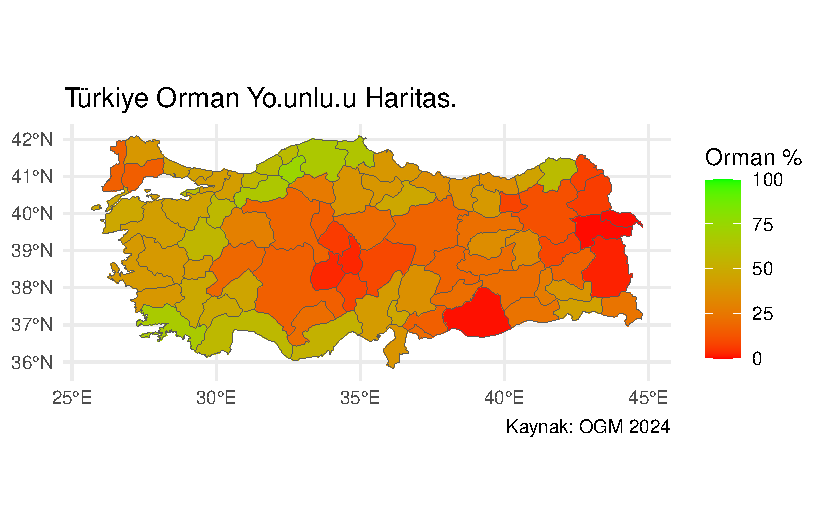
\includegraphics[keepaspectratio]{analysis_files/figure-pdf/unnamed-chunk-9-1.pdf}}

\section{FORESTS FIRES NUMBERS AND AREA ANALYSIS BY
CITIES}\label{forests-fires-numbers-and-area-analysis-by-cities}

\section{This is the part from the previos data.qmd
file}\label{this-is-the-part-from-the-previos-data.qmd-file}

\begin{Shaded}
\begin{Highlighting}[]
\FunctionTok{library}\NormalTok{(sf)}
\FunctionTok{library}\NormalTok{(tidyverse)}
\FunctionTok{library}\NormalTok{(readxl)}
\FunctionTok{library}\NormalTok{(scales) }

\NormalTok{harita\_yolu }\OtherTok{\textless{}{-}} \StringTok{"/Users/zzunb/Downloads/tr{-}cities.json"}
\NormalTok{adet\_yolu }\OtherTok{\textless{}{-}} \StringTok{"/Users/zzunb/Downloads/illere\_gore\_yangin\_adet\_2004{-}2024.xlsx"}
\NormalTok{alan\_yolu }\OtherTok{\textless{}{-}} \StringTok{"/Users/zzunb/Downloads/illere\_gore\_yanan\_alan\_2004{-}2024.xlsx"}

\NormalTok{tr\_map }\OtherTok{\textless{}{-}} \FunctionTok{read\_sf}\NormalTok{(harita\_yolu)}
\NormalTok{df\_adet\_ham }\OtherTok{\textless{}{-}} \FunctionTok{read\_excel}\NormalTok{(adet\_yolu, }\AttributeTok{skip =} \DecValTok{3}\NormalTok{)}
\FunctionTok{colnames}\NormalTok{(df\_adet\_ham)[}\DecValTok{1}\NormalTok{] }\OtherTok{\textless{}{-}} \StringTok{"Bolge"}
\NormalTok{df\_adet\_ham }\OtherTok{\textless{}{-}}\NormalTok{ df\_adet\_ham }\SpecialCharTok{\%\textgreater{}\%} 
  \FunctionTok{filter}\NormalTok{(}\SpecialCharTok{!}\FunctionTok{is.na}\NormalTok{(Bolge)) }\SpecialCharTok{\%\textgreater{}\%} 
  \FunctionTok{slice}\NormalTok{(}\DecValTok{1}\SpecialCharTok{:}\NormalTok{(}\FunctionTok{which}\NormalTok{(Bolge }\SpecialCharTok{==} \StringTok{"Zonguldak"}\NormalTok{))) }\SpecialCharTok{\%\textgreater{}\%}
  \FunctionTok{mutate}\NormalTok{(}\FunctionTok{across}\NormalTok{(}\SpecialCharTok{{-}}\NormalTok{Bolge, }\SpecialCharTok{\textasciitilde{}} \FunctionTok{suppressWarnings}\NormalTok{(}\FunctionTok{as.numeric}\NormalTok{(.))))}

\NormalTok{df\_alan\_ham }\OtherTok{\textless{}{-}} \FunctionTok{read\_excel}\NormalTok{(alan\_yolu, }\AttributeTok{skip =} \DecValTok{3}\NormalTok{)}
\FunctionTok{colnames}\NormalTok{(df\_alan\_ham)[}\DecValTok{1}\NormalTok{] }\OtherTok{\textless{}{-}} \StringTok{"Bolge"}
\NormalTok{df\_alan\_ham }\OtherTok{\textless{}{-}}\NormalTok{ df\_alan\_ham }\SpecialCharTok{\%\textgreater{}\%} 
  \FunctionTok{filter}\NormalTok{(}\SpecialCharTok{!}\FunctionTok{is.na}\NormalTok{(Bolge)) }\SpecialCharTok{\%\textgreater{}\%} 
  \FunctionTok{slice}\NormalTok{(}\DecValTok{1}\SpecialCharTok{:}\NormalTok{(}\FunctionTok{which}\NormalTok{(Bolge }\SpecialCharTok{==} \StringTok{"Zonguldak"}\NormalTok{))) }\SpecialCharTok{\%\textgreater{}\%}
  \FunctionTok{mutate}\NormalTok{(}\FunctionTok{across}\NormalTok{(}\SpecialCharTok{{-}}\NormalTok{Bolge, }\SpecialCharTok{\textasciitilde{}} \FunctionTok{suppressWarnings}\NormalTok{(}\FunctionTok{as.numeric}\NormalTok{(.))))}

\NormalTok{temizle\_ve\_topla }\OtherTok{\textless{}{-}} \ControlFlowTok{function}\NormalTok{(df) \{}
\NormalTok{  df\_sonuc }\OtherTok{\textless{}{-}}\NormalTok{ df }\SpecialCharTok{\%\textgreater{}\%} 
    \FunctionTok{filter}\NormalTok{(}\SpecialCharTok{!}\NormalTok{Bolge }\SpecialCharTok{\%in\%} \FunctionTok{c}\NormalTok{(}\StringTok{"Toplam{-}Total"}\NormalTok{, }\StringTok{"DKMPGM"}\NormalTok{)) }\SpecialCharTok{\%\textgreater{}\%}
    \FunctionTok{mutate}\NormalTok{(}\AttributeTok{Bolge =} \FunctionTok{recode}\NormalTok{(Bolge, }\StringTok{"K.Maraş"} \OtherTok{=} \StringTok{"Kahramanmaraş"}\NormalTok{, }\StringTok{"Afyon"} \OtherTok{=} \StringTok{"Afyonkarahisar"}\NormalTok{)) }\SpecialCharTok{\%\textgreater{}\%}
    \FunctionTok{rowwise}\NormalTok{() }\SpecialCharTok{\%\textgreater{}\%}
    \FunctionTok{mutate}\NormalTok{(}\AttributeTok{Toplam\_21\_Yil =} \FunctionTok{sum}\NormalTok{(}\FunctionTok{c\_across}\NormalTok{(}\FunctionTok{where}\NormalTok{(is.numeric)), }\AttributeTok{na.rm =} \ConstantTok{TRUE}\NormalTok{)) }\SpecialCharTok{\%\textgreater{}\%}
    \FunctionTok{ungroup}\NormalTok{()}
  
  \FunctionTok{return}\NormalTok{(df\_sonuc)}
\NormalTok{\}}

\NormalTok{df\_adet }\OtherTok{\textless{}{-}} \FunctionTok{temizle\_ve\_topla}\NormalTok{(df\_adet\_ham) }\SpecialCharTok{\%\textgreater{}\%} \FunctionTok{arrange}\NormalTok{(}\FunctionTok{desc}\NormalTok{(Toplam\_21\_Yil))}
\NormalTok{df\_alan }\OtherTok{\textless{}{-}} \FunctionTok{temizle\_ve\_topla}\NormalTok{(df\_alan\_ham) }\SpecialCharTok{\%\textgreater{}\%} \FunctionTok{arrange}\NormalTok{(}\FunctionTok{desc}\NormalTok{(Toplam\_21\_Yil))}
\end{Highlighting}
\end{Shaded}

\section{1. time series analysis/line
graphs}\label{time-series-analysisline-graphs}

\begin{Shaded}
\begin{Highlighting}[]
\NormalTok{p1 }\OtherTok{\textless{}{-}}\NormalTok{ df\_adet\_ham }\SpecialCharTok{\%\textgreater{}\%}
  \FunctionTok{filter}\NormalTok{(Bolge }\SpecialCharTok{==} \StringTok{"Toplam{-}Total"}\NormalTok{) }\SpecialCharTok{\%\textgreater{}\%}
  \FunctionTok{pivot\_longer}\NormalTok{(}\AttributeTok{cols =} \SpecialCharTok{{-}}\NormalTok{Bolge, }\AttributeTok{names\_to =} \StringTok{"Yil"}\NormalTok{, }\AttributeTok{values\_to =} \StringTok{"Deger"}\NormalTok{) }\SpecialCharTok{\%\textgreater{}\%}
  \FunctionTok{mutate}\NormalTok{(}\AttributeTok{Yil =} \FunctionTok{as.numeric}\NormalTok{(Yil)) }\SpecialCharTok{\%\textgreater{}\%}
  \FunctionTok{filter}\NormalTok{(}\SpecialCharTok{!}\FunctionTok{is.na}\NormalTok{(Yil)) }\SpecialCharTok{\%\textgreater{}\%}
  \FunctionTok{ggplot}\NormalTok{(}\FunctionTok{aes}\NormalTok{(}\AttributeTok{x =}\NormalTok{ Yil, }\AttributeTok{y =}\NormalTok{ Deger)) }\SpecialCharTok{+}
  \FunctionTok{geom\_line}\NormalTok{(}\AttributeTok{color =} \StringTok{"\#E69F00"}\NormalTok{, }\AttributeTok{size =} \FloatTok{1.2}\NormalTok{) }\SpecialCharTok{+}
  \FunctionTok{geom\_point}\NormalTok{(}\AttributeTok{color =} \StringTok{"black"}\NormalTok{, }\AttributeTok{size =} \DecValTok{2}\NormalTok{) }\SpecialCharTok{+}
  \FunctionTok{geom\_smooth}\NormalTok{(}\AttributeTok{method =} \StringTok{"lm"}\NormalTok{, }\AttributeTok{color =} \StringTok{"blue"}\NormalTok{, }\AttributeTok{linetype =} \StringTok{"dashed"}\NormalTok{, }\AttributeTok{se =} \ConstantTok{FALSE}\NormalTok{, }\AttributeTok{size =} \DecValTok{1}\NormalTok{) }\SpecialCharTok{+} 
  \FunctionTok{scale\_x\_continuous}\NormalTok{(}\AttributeTok{breaks =} \FunctionTok{seq}\NormalTok{(}\DecValTok{2004}\NormalTok{, }\DecValTok{2024}\NormalTok{, }\AttributeTok{by =} \DecValTok{2}\NormalTok{)) }\SpecialCharTok{+}
  \FunctionTok{theme\_minimal}\NormalTok{() }\SpecialCharTok{+}
  \FunctionTok{labs}\NormalTok{(}\AttributeTok{title =} \StringTok{"Yillara Gore Toplam Yangin Adeti (2004{-}2024)"}\NormalTok{, }
       \AttributeTok{subtitle =} \StringTok{"Mavi kesik cizgi genel artis/azalis egilimini gosterir."}\NormalTok{,}
       \AttributeTok{x =} \StringTok{"Yil"}\NormalTok{, }\AttributeTok{y =} \StringTok{"Yangin Adeti"}\NormalTok{)}
\end{Highlighting}
\end{Shaded}

\begin{verbatim}
Warning: Using `size` aesthetic for lines was deprecated in ggplot2 3.4.0.
i Please use `linewidth` instead.
\end{verbatim}

\section{2. merging map and data}\label{merging-map-and-data}

\begin{Shaded}
\begin{Highlighting}[]
\NormalTok{p2 }\OtherTok{\textless{}{-}}\NormalTok{ df\_alan\_ham }\SpecialCharTok{\%\textgreater{}\%}
  \FunctionTok{filter}\NormalTok{(Bolge }\SpecialCharTok{==} \StringTok{"Toplam{-}Total"}\NormalTok{) }\SpecialCharTok{\%\textgreater{}\%}
  \FunctionTok{pivot\_longer}\NormalTok{(}\AttributeTok{cols =} \SpecialCharTok{{-}}\NormalTok{Bolge, }\AttributeTok{names\_to =} \StringTok{"Yil"}\NormalTok{, }\AttributeTok{values\_to =} \StringTok{"Deger"}\NormalTok{) }\SpecialCharTok{\%\textgreater{}\%}
  \FunctionTok{mutate}\NormalTok{(}\AttributeTok{Yil =} \FunctionTok{as.numeric}\NormalTok{(Yil)) }\SpecialCharTok{\%\textgreater{}\%}
  \FunctionTok{filter}\NormalTok{(}\SpecialCharTok{!}\FunctionTok{is.na}\NormalTok{(Yil)) }\SpecialCharTok{\%\textgreater{}\%}
  \FunctionTok{ggplot}\NormalTok{(}\FunctionTok{aes}\NormalTok{(}\AttributeTok{x =}\NormalTok{ Yil, }\AttributeTok{y =}\NormalTok{ Deger)) }\SpecialCharTok{+}
  \FunctionTok{geom\_line}\NormalTok{(}\AttributeTok{color =} \StringTok{"\#D55E00"}\NormalTok{, }\AttributeTok{size =} \FloatTok{1.2}\NormalTok{) }\SpecialCharTok{+}
  \FunctionTok{geom\_point}\NormalTok{(}\AttributeTok{color =} \StringTok{"black"}\NormalTok{, }\AttributeTok{size =} \DecValTok{2}\NormalTok{) }\SpecialCharTok{+}
  \FunctionTok{annotate}\NormalTok{(}\StringTok{"text"}\NormalTok{, }\AttributeTok{x =} \DecValTok{2016}\NormalTok{, }\AttributeTok{y =} \DecValTok{125000}\NormalTok{, }\AttributeTok{label =} \StringTok{"2021 Yili Dev Yanginlari:}\SpecialCharTok{\textbackslash{}n}\StringTok{\textasciitilde{}139.503 Hektar"}\NormalTok{, }\AttributeTok{color =} \StringTok{"red"}\NormalTok{, }\AttributeTok{fontface =} \StringTok{"bold"}\NormalTok{) }\SpecialCharTok{+}
  \FunctionTok{annotate}\NormalTok{(}\StringTok{"curve"}\NormalTok{, }\AttributeTok{x =} \DecValTok{2018}\NormalTok{, }\AttributeTok{y =} \DecValTok{125000}\NormalTok{, }\AttributeTok{xend =} \FloatTok{2020.8}\NormalTok{, }\AttributeTok{yend =} \DecValTok{139500}\NormalTok{, }
           \AttributeTok{arrow =} \FunctionTok{arrow}\NormalTok{(}\AttributeTok{length =} \FunctionTok{unit}\NormalTok{(}\FloatTok{0.3}\NormalTok{, }\StringTok{"cm"}\NormalTok{)), }\AttributeTok{curvature =} \SpecialCharTok{{-}}\FloatTok{0.3}\NormalTok{, }\AttributeTok{color =} \StringTok{"red"}\NormalTok{, }\AttributeTok{size =} \DecValTok{1}\NormalTok{) }\SpecialCharTok{+}
  \FunctionTok{scale\_x\_continuous}\NormalTok{(}\AttributeTok{breaks =} \FunctionTok{seq}\NormalTok{(}\DecValTok{2004}\NormalTok{, }\DecValTok{2024}\NormalTok{, }\AttributeTok{by =} \DecValTok{2}\NormalTok{)) }\SpecialCharTok{+}
  \FunctionTok{scale\_y\_continuous}\NormalTok{(}\AttributeTok{labels =} \FunctionTok{label\_number}\NormalTok{(}\AttributeTok{big.mark =} \StringTok{"."}\NormalTok{, }\AttributeTok{decimal.mark =} \StringTok{","}\NormalTok{)) }\SpecialCharTok{+} 
  \FunctionTok{theme\_minimal}\NormalTok{() }\SpecialCharTok{+}
  \FunctionTok{labs}\NormalTok{(}\AttributeTok{title =} \StringTok{"Yillara Gore Toplam Yanan Alan (2004{-}2024)"}\NormalTok{, }\AttributeTok{x =} \StringTok{"Yil"}\NormalTok{, }\AttributeTok{y =} \StringTok{"Hektar Alan"}\NormalTok{)}

\FunctionTok{print}\NormalTok{(p1)}
\end{Highlighting}
\end{Shaded}

\begin{verbatim}
`geom_smooth()` using formula = 'y ~ x'
\end{verbatim}

\pandocbounded{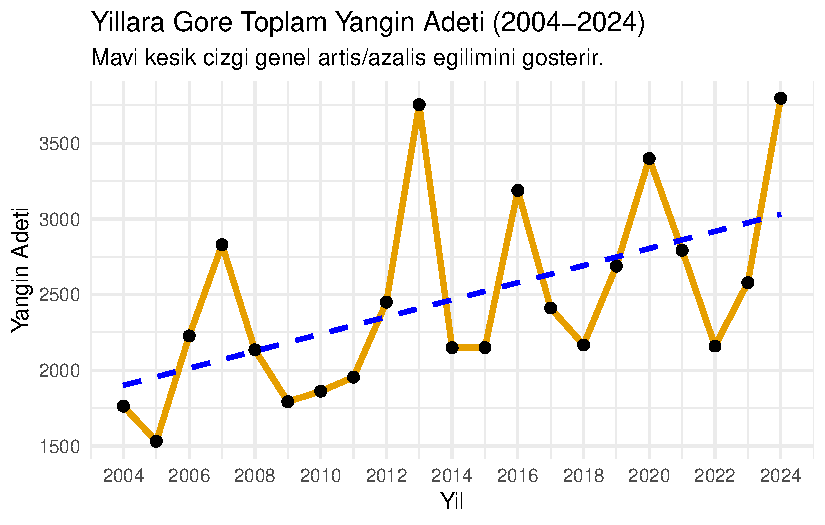
\includegraphics[keepaspectratio]{analysis_files/figure-pdf/unnamed-chunk-12-1.pdf}}

\begin{Shaded}
\begin{Highlighting}[]
\FunctionTok{print}\NormalTok{(p2)}
\end{Highlighting}
\end{Shaded}

\pandocbounded{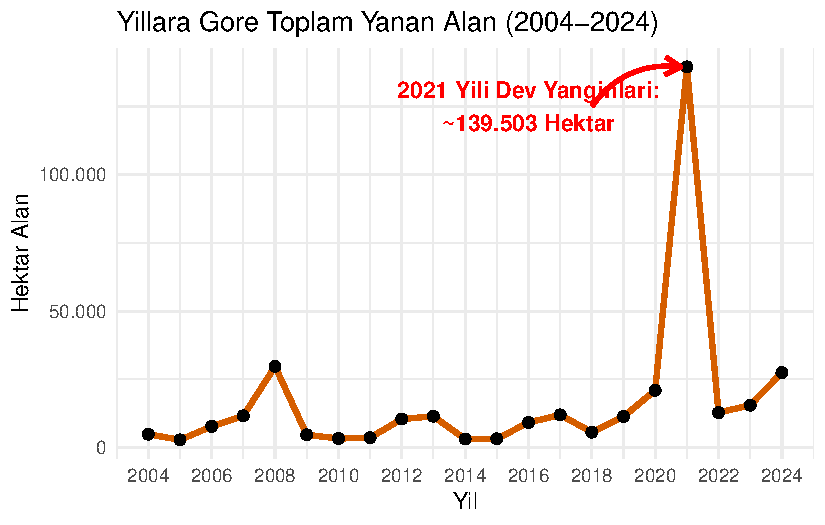
\includegraphics[keepaspectratio]{analysis_files/figure-pdf/unnamed-chunk-12-2.pdf}}

\section{3.drawing the map-data
visualization}\label{drawing-the-map-data-visualization}

\begin{Shaded}
\begin{Highlighting}[]
\NormalTok{harita\_adet }\OtherTok{\textless{}{-}}\NormalTok{ tr\_map }\SpecialCharTok{\%\textgreater{}\%} \FunctionTok{left\_join}\NormalTok{(df\_adet, }\AttributeTok{by =} \FunctionTok{c}\NormalTok{(}\StringTok{"name"} \OtherTok{=} \StringTok{"Bolge"}\NormalTok{))}

\NormalTok{g1 }\OtherTok{\textless{}{-}} \FunctionTok{ggplot}\NormalTok{(}\AttributeTok{data =}\NormalTok{ harita\_adet) }\SpecialCharTok{+}
  \FunctionTok{geom\_sf}\NormalTok{(}\FunctionTok{aes}\NormalTok{(}\AttributeTok{fill =}\NormalTok{ Toplam\_21\_Yil), }\AttributeTok{color =} \StringTok{"black"}\NormalTok{, }\AttributeTok{size =} \FloatTok{0.2}\NormalTok{) }\SpecialCharTok{+}
  \FunctionTok{stat\_sf\_coordinates}\NormalTok{(}\FunctionTok{aes}\NormalTok{(}\AttributeTok{label =}\NormalTok{ name), }\AttributeTok{geom =} \StringTok{"text"}\NormalTok{, }\AttributeTok{size =} \FloatTok{2.2}\NormalTok{, }\AttributeTok{color =} \StringTok{"black"}\NormalTok{, }\AttributeTok{fontface =} \StringTok{"bold"}\NormalTok{, }\AttributeTok{check\_overlap =} \ConstantTok{TRUE}\NormalTok{) }\SpecialCharTok{+}
  \FunctionTok{scale\_fill\_gradientn}\NormalTok{(}\AttributeTok{colors =} \FunctionTok{c}\NormalTok{(}\StringTok{"\#00BA38"}\NormalTok{, }\StringTok{"yellow"}\NormalTok{, }\StringTok{"\#F8766D"}\NormalTok{, }\StringTok{"\#B71C1C"}\NormalTok{), }\AttributeTok{name =} \StringTok{"Toplam Adet"}\NormalTok{, }\AttributeTok{na.value =} \StringTok{"gray90"}\NormalTok{) }\SpecialCharTok{+}
  \FunctionTok{theme\_void}\NormalTok{() }\SpecialCharTok{+}
  \FunctionTok{theme}\NormalTok{(}
    \AttributeTok{plot.margin =} \FunctionTok{margin}\NormalTok{(}\AttributeTok{t =} \DecValTok{20}\NormalTok{, }\AttributeTok{r =} \DecValTok{20}\NormalTok{, }\AttributeTok{b =} \DecValTok{20}\NormalTok{, }\AttributeTok{l =} \DecValTok{20}\NormalTok{, }\AttributeTok{unit =} \StringTok{"pt"}\NormalTok{), }
    \AttributeTok{plot.title =} \FunctionTok{element\_text}\NormalTok{(}\AttributeTok{hjust =} \FloatTok{0.5}\NormalTok{, }\AttributeTok{face =} \StringTok{"bold"}\NormalTok{, }\AttributeTok{size =} \DecValTok{14}\NormalTok{, }\AttributeTok{margin =} \FunctionTok{margin}\NormalTok{(}\AttributeTok{b =} \DecValTok{15}\NormalTok{)), }
    \AttributeTok{plot.caption =} \FunctionTok{element\_text}\NormalTok{(}\AttributeTok{hjust =} \DecValTok{1}\NormalTok{, }\AttributeTok{margin =} \FunctionTok{margin}\NormalTok{(}\AttributeTok{t =} \DecValTok{10}\NormalTok{), }\AttributeTok{lineheight =} \FloatTok{1.2}\NormalTok{), }\CommentTok{\# SatD1r aralD1DD1 eklendi}
    \AttributeTok{legend.margin =} \FunctionTok{margin}\NormalTok{(}\AttributeTok{l =} \DecValTok{10}\NormalTok{, }\AttributeTok{r =} \DecValTok{10}\NormalTok{) }
\NormalTok{  ) }\SpecialCharTok{+}
  \FunctionTok{labs}\NormalTok{(}
    \AttributeTok{title =} \StringTok{"Illere Gore Toplam Yangin Sayisi (2004{-}2024)"}\NormalTok{, }
    \AttributeTok{caption =} \StringTok{"Veriler: OGM}\SpecialCharTok{\textbackslash{}n}\StringTok{Gri renkteki iller icin veri bulunmamaktadir."}
\NormalTok{  )}

\NormalTok{harita\_alan }\OtherTok{\textless{}{-}}\NormalTok{ tr\_map }\SpecialCharTok{\%\textgreater{}\%} \FunctionTok{left\_join}\NormalTok{(df\_alan, }\AttributeTok{by =} \FunctionTok{c}\NormalTok{(}\StringTok{"name"} \OtherTok{=} \StringTok{"Bolge"}\NormalTok{))}

\NormalTok{g2 }\OtherTok{\textless{}{-}} \FunctionTok{ggplot}\NormalTok{(}\AttributeTok{data =}\NormalTok{ harita\_alan) }\SpecialCharTok{+}
  \FunctionTok{geom\_sf}\NormalTok{(}\FunctionTok{aes}\NormalTok{(}\AttributeTok{fill =}\NormalTok{ Toplam\_21\_Yil), }\AttributeTok{color =} \StringTok{"black"}\NormalTok{, }\AttributeTok{size =} \FloatTok{0.2}\NormalTok{) }\SpecialCharTok{+}
  \FunctionTok{stat\_sf\_coordinates}\NormalTok{(}\FunctionTok{aes}\NormalTok{(}\AttributeTok{label =}\NormalTok{ name), }\AttributeTok{geom =} \StringTok{"text"}\NormalTok{, }\AttributeTok{size =} \FloatTok{2.2}\NormalTok{, }\AttributeTok{color =} \StringTok{"black"}\NormalTok{, }\AttributeTok{fontface =} \StringTok{"bold"}\NormalTok{, }\AttributeTok{check\_overlap =} \ConstantTok{TRUE}\NormalTok{) }\SpecialCharTok{+}
  \FunctionTok{scale\_fill\_gradientn}\NormalTok{(}
    \AttributeTok{colors =} \FunctionTok{c}\NormalTok{(}\StringTok{"\#00BA38"}\NormalTok{, }\StringTok{"yellow"}\NormalTok{, }\StringTok{"\#F8766D"}\NormalTok{, }\StringTok{"\#B71C1C"}\NormalTok{), }
    \AttributeTok{trans =} \StringTok{"pseudo\_log"}\NormalTok{, }
    \AttributeTok{breaks =} \FunctionTok{c}\NormalTok{(}\DecValTok{100}\NormalTok{, }\DecValTok{1000}\NormalTok{, }\DecValTok{10000}\NormalTok{, }\DecValTok{100000}\NormalTok{), }
    \AttributeTok{labels =} \FunctionTok{c}\NormalTok{(}\StringTok{"100"}\NormalTok{, }\StringTok{"1.000"}\NormalTok{, }\StringTok{"10.000"}\NormalTok{, }\StringTok{"100.000+"}\NormalTok{), }
    \AttributeTok{name =} \StringTok{"Toplam Hektar}\SpecialCharTok{\textbackslash{}n}\StringTok{(Log Skala)"}\NormalTok{, }
    \AttributeTok{na.value =} \StringTok{"gray90"}
\NormalTok{  ) }\SpecialCharTok{+}
  \FunctionTok{theme\_void}\NormalTok{() }\SpecialCharTok{+}
  \FunctionTok{theme}\NormalTok{(}
    \AttributeTok{plot.margin =} \FunctionTok{margin}\NormalTok{(}\AttributeTok{t =} \DecValTok{20}\NormalTok{, }\AttributeTok{r =} \DecValTok{20}\NormalTok{, }\AttributeTok{b =} \DecValTok{20}\NormalTok{, }\AttributeTok{l =} \DecValTok{20}\NormalTok{, }\AttributeTok{unit =} \StringTok{"pt"}\NormalTok{), }
    \AttributeTok{plot.title =} \FunctionTok{element\_text}\NormalTok{(}\AttributeTok{hjust =} \FloatTok{0.5}\NormalTok{, }\AttributeTok{face =} \StringTok{"bold"}\NormalTok{, }\AttributeTok{size =} \DecValTok{14}\NormalTok{, }\AttributeTok{margin =} \FunctionTok{margin}\NormalTok{(}\AttributeTok{b =} \DecValTok{15}\NormalTok{)), }
    \AttributeTok{plot.caption =} \FunctionTok{element\_text}\NormalTok{(}\AttributeTok{hjust =} \DecValTok{1}\NormalTok{, }\AttributeTok{margin =} \FunctionTok{margin}\NormalTok{(}\AttributeTok{t =} \DecValTok{10}\NormalTok{), }\AttributeTok{lineheight =} \FloatTok{1.2}\NormalTok{), }\CommentTok{\# SatD1r aralD1DD1 eklendi}
    \AttributeTok{legend.margin =} \FunctionTok{margin}\NormalTok{(}\AttributeTok{l =} \DecValTok{10}\NormalTok{, }\AttributeTok{r =} \DecValTok{10}\NormalTok{) }
\NormalTok{  ) }\SpecialCharTok{+}
  \FunctionTok{labs}\NormalTok{(}
    \AttributeTok{title =} \StringTok{"Illere Gore Toplam Yanan Alan (Hektar) (2004{-}2024)"}\NormalTok{, }
    \AttributeTok{caption =} \StringTok{"Veriler: OGM}\SpecialCharTok{\textbackslash{}n}\StringTok{Gri renkteki iller icin veri bulunmamaktadir."}
\NormalTok{  )}

\FunctionTok{print}\NormalTok{(g1)}
\end{Highlighting}
\end{Shaded}

\begin{verbatim}
Warning in st_point_on_surface.sfc(sf::st_zm(x)): st_point_on_surface may not
give correct results for longitude/latitude data
\end{verbatim}

\pandocbounded{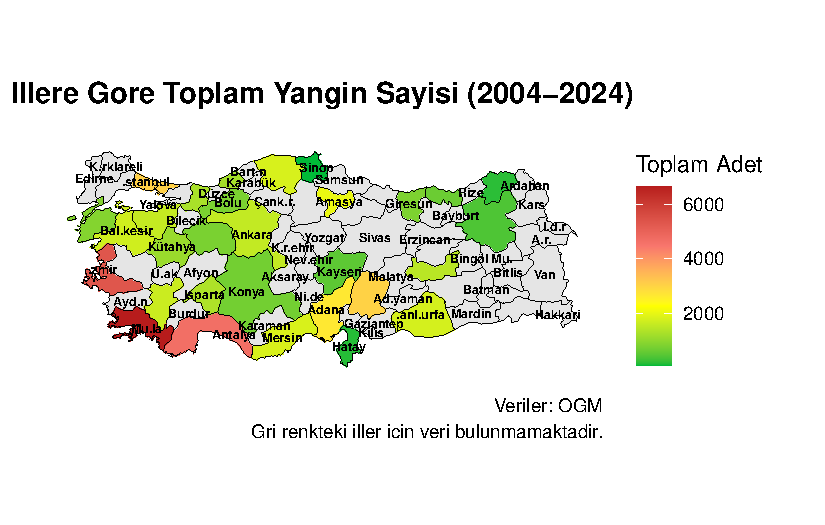
\includegraphics[keepaspectratio]{analysis_files/figure-pdf/unnamed-chunk-13-1.pdf}}

\begin{Shaded}
\begin{Highlighting}[]
\FunctionTok{print}\NormalTok{(g2)}
\end{Highlighting}
\end{Shaded}

\begin{verbatim}
Warning in st_point_on_surface.sfc(sf::st_zm(x)): st_point_on_surface may not
give correct results for longitude/latitude data
\end{verbatim}

\pandocbounded{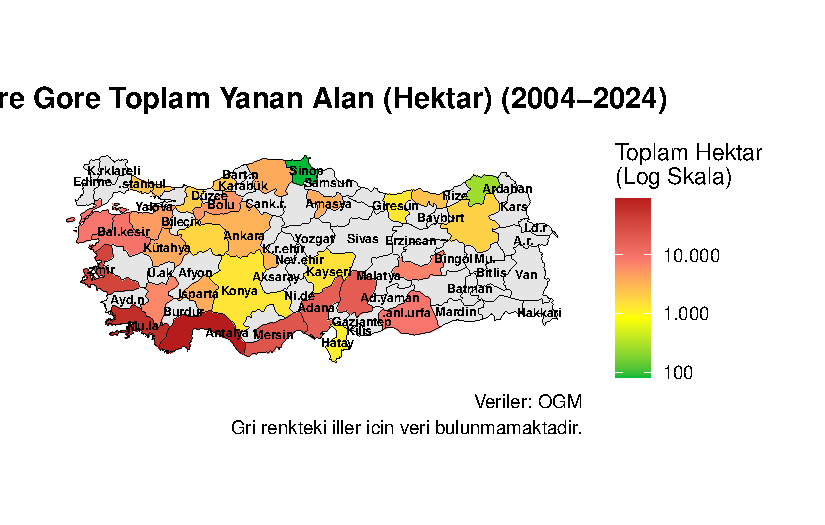
\includegraphics[keepaspectratio]{analysis_files/figure-pdf/unnamed-chunk-13-2.pdf}}

\section{FOREST FIRES CAUSING MAIN
REASONS}\label{forest-fires-causing-main-reasons}

\section{This is the part from the previos data.qmd
file}\label{this-is-the-part-from-the-previos-data.qmd-file-1}

\begin{Shaded}
\begin{Highlighting}[]
\FunctionTok{library}\NormalTok{(sf)}
\FunctionTok{library}\NormalTok{(tidyverse)}
\FunctionTok{library}\NormalTok{(readxl)}

\NormalTok{harita\_yolu }\OtherTok{\textless{}{-}} \StringTok{"/Users/zzunb/Downloads/tr{-}cities.json"}
\NormalTok{excel\_yolu }\OtherTok{\textless{}{-}} \StringTok{"/Users/zzunb/Downloads/2022{-}2024\_sebep\_adet\_toplam.xlsx"}

\NormalTok{tr\_map }\OtherTok{\textless{}{-}} \FunctionTok{read\_sf}\NormalTok{(harita\_yolu)}

\NormalTok{yangin\_verisi }\OtherTok{\textless{}{-}} \FunctionTok{read\_excel}\NormalTok{(excel\_yolu, }\AttributeTok{skip =} \DecValTok{5}\NormalTok{, }\AttributeTok{n\_max =} \DecValTok{31}\NormalTok{, }\AttributeTok{col\_names =} \ConstantTok{FALSE}\NormalTok{) }\SpecialCharTok{\%\textgreater{}\%}
  \FunctionTok{select}\NormalTok{(}
    \AttributeTok{Bolge =} \DecValTok{1}\NormalTok{,}
    \AttributeTok{Aniz =} \DecValTok{2}\NormalTok{, }\AttributeTok{Coplu =} \DecValTok{3}\NormalTok{, }\AttributeTok{Avcilik =} \DecValTok{4}\NormalTok{, }\AttributeTok{CobanAtesi =} \DecValTok{5}\NormalTok{, }\AttributeTok{Sigara =} \DecValTok{6}\NormalTok{, }\AttributeTok{Piknik =} \DecValTok{7}\NormalTok{, }\AttributeTok{Diger\_Ihmal =} \DecValTok{8}\NormalTok{,}
    \AttributeTok{Teror =} \DecValTok{10}\NormalTok{, }\AttributeTok{Kundaklama =} \DecValTok{11}\NormalTok{, }\AttributeTok{Acma =} \DecValTok{12}\NormalTok{, }\AttributeTok{Diger\_Kasit =} \DecValTok{13}\NormalTok{,}
    \AttributeTok{Enerji =} \DecValTok{15}\NormalTok{, }\AttributeTok{Trafik =} \DecValTok{16}\NormalTok{, }\AttributeTok{Diger\_Kaza =} \DecValTok{17}\NormalTok{,}
    \AttributeTok{Bilinmeyen =} \DecValTok{19}\NormalTok{, }\AttributeTok{Dogal =} \DecValTok{20}
\NormalTok{  ) }\SpecialCharTok{\%\textgreater{}\%}
  \FunctionTok{mutate}\NormalTok{(}\FunctionTok{across}\NormalTok{(}\SpecialCharTok{{-}}\NormalTok{Bolge, }\SpecialCharTok{\textasciitilde{}}\FunctionTok{as.numeric}\NormalTok{(}\FunctionTok{ifelse}\NormalTok{(. }\SpecialCharTok{==} \StringTok{"{-}"}\NormalTok{, }\StringTok{"0"}\NormalTok{, .)))) }\SpecialCharTok{\%\textgreater{}\%}
  \FunctionTok{filter}\NormalTok{(}\SpecialCharTok{!}\NormalTok{Bolge }\SpecialCharTok{\%in\%} \FunctionTok{c}\NormalTok{(}\StringTok{"DKMPGM"}\NormalTok{, }\StringTok{"Toplam{-}Total"}\NormalTok{))}

\NormalTok{yangin\_verisi }\OtherTok{\textless{}{-}}\NormalTok{ yangin\_verisi }\SpecialCharTok{\%\textgreater{}\%}
  \FunctionTok{mutate}\NormalTok{(}\AttributeTok{Bolge =} \FunctionTok{recode}\NormalTok{(Bolge, }
                        \StringTok{"K.MaraE"} \OtherTok{=} \StringTok{"KahramanmaraE"}\NormalTok{,}
                        \StringTok{"Afyon"} \OtherTok{=} \StringTok{"Afyonkarahisar"}\NormalTok{))}
\end{Highlighting}
\end{Shaded}

\section{1. determining the dominant reason of
fires}\label{determining-the-dominant-reason-of-fires}

\begin{Shaded}
\begin{Highlighting}[]
\NormalTok{baskin\_analiz }\OtherTok{\textless{}{-}}\NormalTok{ yangin\_verisi }\SpecialCharTok{\%\textgreater{}\%}
  \FunctionTok{pivot\_longer}\NormalTok{(}\AttributeTok{cols =} \SpecialCharTok{{-}}\NormalTok{Bolge, }\AttributeTok{names\_to =} \StringTok{"Alt\_Sebep"}\NormalTok{, }\AttributeTok{values\_to =} \StringTok{"Miktar"}\NormalTok{) }\SpecialCharTok{\%\textgreater{}\%}
  \FunctionTok{group\_by}\NormalTok{(Bolge) }\SpecialCharTok{\%\textgreater{}\%}
  \FunctionTok{slice\_max}\NormalTok{(}\AttributeTok{order\_by =}\NormalTok{ Miktar, }\AttributeTok{n =} \DecValTok{1}\NormalTok{, }\AttributeTok{with\_ties =} \ConstantTok{FALSE}\NormalTok{) }\SpecialCharTok{\%\textgreater{}\%}
  \FunctionTok{ungroup}\NormalTok{() }\SpecialCharTok{\%\textgreater{}\%}
  \CommentTok{\# 5. AdD1mdaki recode kD1smD1nD1 Eununla gC\textless{}ncelle:}
  \FunctionTok{mutate}\NormalTok{(}\AttributeTok{Alt\_Sebep =} \FunctionTok{recode}\NormalTok{(Alt\_Sebep, }
                            \StringTok{"Bilinmeyen"} \OtherTok{=} \StringTok{"Sebebi Bilinmeyen"}\NormalTok{,}
                            \StringTok{"Dogal"} \OtherTok{=} \StringTok{"Dogal (Yildirim)"}\NormalTok{,}
                            \StringTok{"Diger\_Ihmal"} \OtherTok{=} \StringTok{"Ihmal(Diger)"}\NormalTok{, }\CommentTok{\# D0sim deDiEti}
                            \StringTok{"Aniz"} \OtherTok{=} \StringTok{"Aniz(Ihmal)"}\NormalTok{,         }\CommentTok{\# D0sim deDiEti}
                            \StringTok{"Diger\_Kasit"} \OtherTok{=} \StringTok{"Diger (Kasit)"}\NormalTok{,}
                            \StringTok{"Diger\_Kaza"} \OtherTok{=} \StringTok{"Diger (Kaza)"}\NormalTok{,}
                            \StringTok{"CobanAtesi"} \OtherTok{=} \StringTok{"Coban Atesi"}\NormalTok{))}
\end{Highlighting}
\end{Shaded}

\section{2. seting the colors of the
categories}\label{seting-the-colors-of-the-categories}

\begin{Shaded}
\begin{Highlighting}[]
\NormalTok{renk\_paleti }\OtherTok{\textless{}{-}} \FunctionTok{c}\NormalTok{(}
  \CommentTok{\# D0HMAL {-} Sadece SarD1 ve AC\textquotesingle{}D1k Turuncu (KD1rmD1zD1dan tamamen baDD1msD1z)}
  \StringTok{"Aniz"} \OtherTok{=} \StringTok{"\#FFFFE5"}\NormalTok{, }\StringTok{"Coplu"} \OtherTok{=} \StringTok{"\#FFF7BC"}\NormalTok{, }\StringTok{"Avcilik"} \OtherTok{=} \StringTok{"\#FEE391"}\NormalTok{, }
  \StringTok{"Coban Atesi"} \OtherTok{=} \StringTok{"\#FEC44F"}\NormalTok{, }\StringTok{"Sigara"} \OtherTok{=} \StringTok{"\#FE9929"}\NormalTok{, }\StringTok{"Piknik"} \OtherTok{=} \StringTok{"\#EC7014"}\NormalTok{, }\StringTok{"Diger (Ihmal)"} \OtherTok{=} \StringTok{"\#CC4C02"}\NormalTok{,}
  
  \CommentTok{\# KASIT {-} Koyu KD1rmD1zD1 ve Bordo TonlarD1}
  \StringTok{"Teror"} \OtherTok{=} \StringTok{"\#FCBBA1"}\NormalTok{, }\StringTok{"Kundaklama"} \OtherTok{=} \StringTok{"\#FB6A4A"}\NormalTok{, }\StringTok{"Acma"} \OtherTok{=} \StringTok{"\#CB181D"}\NormalTok{, }\StringTok{"Diger (Kasit)"} \OtherTok{=} \StringTok{"\#67000D"}\NormalTok{,}
  
  \CommentTok{\# KAZA {-} Saf Mavi TonlarD1}
  \StringTok{"Enerji"} \OtherTok{=} \StringTok{"\#DEEBF7"}\NormalTok{, }\StringTok{"Trafik"} \OtherTok{=} \StringTok{"\#6BAED6"}\NormalTok{, }\StringTok{"Diger (Kaza)"} \OtherTok{=} \StringTok{"\#08306B"}\NormalTok{,}
  
  \CommentTok{\# SEBEBD0 BD0LD0NMEYEN {-} Mor}
  \StringTok{"Sebebi Bilinmeyen"} \OtherTok{=} \StringTok{"\#9467BD"}\NormalTok{,}
  
  \CommentTok{\# DODAL {-} YeEil}
  \StringTok{"Dogal (Yildirim)"} \OtherTok{=} \StringTok{"\#2CA02C"}
\NormalTok{)}
\end{Highlighting}
\end{Shaded}

\section{3. drawing the final map of the
causes}\label{drawing-the-final-map-of-the-causes}

\begin{Shaded}
\begin{Highlighting}[]
\NormalTok{harita\_final }\OtherTok{\textless{}{-}}\NormalTok{ tr\_map }\SpecialCharTok{\%\textgreater{}\%}
  \FunctionTok{left\_join}\NormalTok{(baskin\_analiz, }\AttributeTok{by =} \FunctionTok{c}\NormalTok{(}\StringTok{"name"} \OtherTok{=} \StringTok{"Bolge"}\NormalTok{))}

\FunctionTok{ggplot}\NormalTok{(}\AttributeTok{data =}\NormalTok{ harita\_final) }\SpecialCharTok{+}
  \FunctionTok{geom\_sf}\NormalTok{(}\FunctionTok{aes}\NormalTok{(}\AttributeTok{fill =}\NormalTok{ Alt\_Sebep), }\AttributeTok{color =} \StringTok{"black"}\NormalTok{, }\AttributeTok{size =} \FloatTok{0.2}\NormalTok{) }\SpecialCharTok{+}
  \CommentTok{\# Il isimleri}
  \FunctionTok{stat\_sf\_coordinates}\NormalTok{(}\FunctionTok{aes}\NormalTok{(}\AttributeTok{label =}\NormalTok{ name), }\AttributeTok{geom =} \StringTok{"text"}\NormalTok{, }\AttributeTok{size =} \FloatTok{2.2}\NormalTok{, }\AttributeTok{color =} \StringTok{"black"}\NormalTok{, }\AttributeTok{fontface =} \StringTok{"bold"}\NormalTok{, }\AttributeTok{check\_overlap =} \ConstantTok{TRUE}\NormalTok{) }\SpecialCharTok{+}
  
  \FunctionTok{scale\_fill\_manual}\NormalTok{(}
    \AttributeTok{values =} \FunctionTok{c}\NormalTok{(}
      \CommentTok{\# IHMAL GRUBU (Sari/Turuncu)}
      \StringTok{"Aniz(Ihmal)"} \OtherTok{=} \StringTok{"\#FFFFE5"}\NormalTok{, }\StringTok{"Coplu"} \OtherTok{=} \StringTok{"\#FFF7BC"}\NormalTok{, }\StringTok{"Avcilik"} \OtherTok{=} \StringTok{"\#FEE391"}\NormalTok{, }
      \StringTok{"Coban Atesi"} \OtherTok{=} \StringTok{"\#FEC44F"}\NormalTok{, }\StringTok{"Sigara"} \OtherTok{=} \StringTok{"\#FE9929"}\NormalTok{, }\StringTok{"Piknik"} \OtherTok{=} \StringTok{"\#FB9A29"}\NormalTok{, }
      \StringTok{"Ihmal(Diger)"} \OtherTok{=} \StringTok{"\#EC7014"}\NormalTok{, }
      
      \CommentTok{\# KASIT GRUBU (Kirmizi)}
      \StringTok{"Teror"} \OtherTok{=} \StringTok{"\#FEE5D9"}\NormalTok{, }\StringTok{"Kundaklama"} \OtherTok{=} \StringTok{"\#FCAE91"}\NormalTok{, }\StringTok{"Acma"} \OtherTok{=} \StringTok{"\#FB6A4A"}\NormalTok{, }\StringTok{"Diger (Kasit)"} \OtherTok{=} \StringTok{"\#CB181D"}\NormalTok{,}
      
      \CommentTok{\# KAZA GRUBU (Mavi)}
      \StringTok{"Enerji"} \OtherTok{=} \StringTok{"\#DEEBF7"}\NormalTok{, }\StringTok{"Trafik"} \OtherTok{=} \StringTok{"\#6BAED6"}\NormalTok{, }\StringTok{"Diger (Kaza)"} \OtherTok{=} \StringTok{"\#08306B"}\NormalTok{,}
      
      \CommentTok{\# DIGERLERI}
      \StringTok{"Sebebi Bilinmeyen"} \OtherTok{=} \StringTok{"\#9467BD"}\NormalTok{,}
      \StringTok{"Dogal (Yildirim)"} \OtherTok{=} \StringTok{"\#2CA02C"}
\NormalTok{    ), }
    \AttributeTok{na.value =} \StringTok{"gray90"}\NormalTok{, }
    \AttributeTok{name =} \StringTok{"Baskin Sebep Detayi"}
\NormalTok{  ) }\SpecialCharTok{+}
  \FunctionTok{theme\_minimal}\NormalTok{() }\SpecialCharTok{+}
  \FunctionTok{theme}\NormalTok{(}
    \AttributeTok{axis.text =} \FunctionTok{element\_blank}\NormalTok{(),}
    \AttributeTok{axis.ticks =} \FunctionTok{element\_blank}\NormalTok{(),}
    \AttributeTok{panel.grid =} \FunctionTok{element\_blank}\NormalTok{(),}
    \AttributeTok{legend.position =} \StringTok{"right"}\NormalTok{,}
    \AttributeTok{legend.title =} \FunctionTok{element\_text}\NormalTok{(}\AttributeTok{face =} \StringTok{"bold"}\NormalTok{, }\AttributeTok{size =} \DecValTok{9}\NormalTok{),}
    \AttributeTok{legend.text =} \FunctionTok{element\_text}\NormalTok{(}\AttributeTok{size =} \DecValTok{8}\NormalTok{),}
    \AttributeTok{plot.title =} \FunctionTok{element\_text}\NormalTok{(}\AttributeTok{hjust =} \FloatTok{0.5}\NormalTok{, }\AttributeTok{face =} \StringTok{"bold"}\NormalTok{, }\AttributeTok{size =} \DecValTok{14}\NormalTok{),}
    \AttributeTok{plot.subtitle =} \FunctionTok{element\_text}\NormalTok{(}\AttributeTok{hjust =} \FloatTok{0.5}\NormalTok{, }\AttributeTok{size =} \DecValTok{10}\NormalTok{, }\AttributeTok{face =} \StringTok{"italic"}\NormalTok{),}
    \AttributeTok{plot.caption =} \FunctionTok{element\_text}\NormalTok{(}\AttributeTok{hjust =} \DecValTok{0}\NormalTok{, }\AttributeTok{size =} \DecValTok{8}\NormalTok{, }\AttributeTok{lineheight =} \FloatTok{1.2}\NormalTok{)}
\NormalTok{  ) }\SpecialCharTok{+}
  \FunctionTok{labs}\NormalTok{(}
    \AttributeTok{title =} \StringTok{"Turkiye Orman Yanginlari Baskin Sebep Analizi (2022{-}2024)"}\NormalTok{,}
    \AttributeTok{subtitle =} \StringTok{"Sari/Turuncu: Ihmal | Kirmizi: Kasit | Mavi: Kaza | Mor: Bilinmeyen | Yesil: Dogal"}\NormalTok{,}
    \AttributeTok{caption =} \FunctionTok{paste0}\NormalTok{(}
      \StringTok{"Veriler Orman Genel Mudurlugune aittir.}\SpecialCharTok{\textbackslash{}n\textbackslash{}n}\StringTok{"}\NormalTok{,}
      \StringTok{"Ihmal(Diger) Kategorisi: Coban/avci atesi, cocuklarin atesle oynamasi, copluk ve tarla temizligi,piknik,sigara gibi nedenleri kapsar.}\SpecialCharTok{\textbackslash{}n\textbackslash{}n}\StringTok{"}\NormalTok{,}
      \StringTok{"Gri alanlar veri seti disinda kalan illeri temsil eder."}
\NormalTok{    )}
\NormalTok{  )}
\end{Highlighting}
\end{Shaded}

\begin{verbatim}
Warning in st_point_on_surface.sfc(sf::st_zm(x)): st_point_on_surface may not
give correct results for longitude/latitude data
\end{verbatim}

\pandocbounded{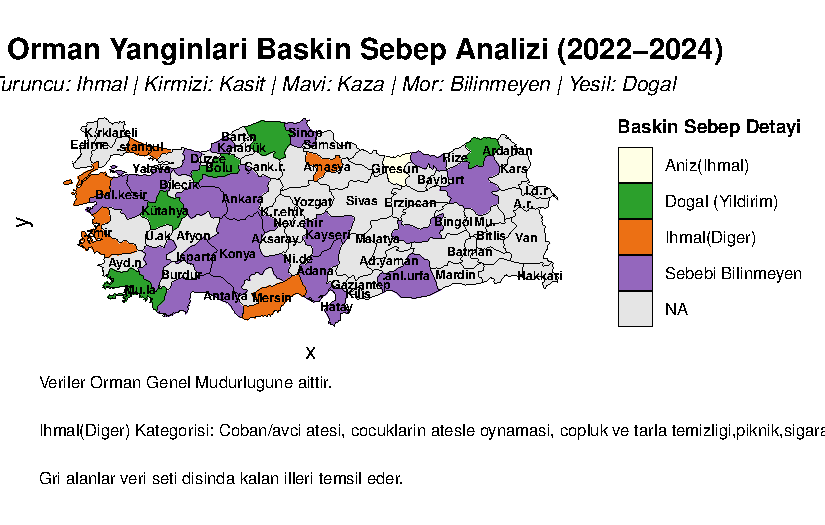
\includegraphics[keepaspectratio]{analysis_files/figure-pdf/unnamed-chunk-17-1.pdf}}

\#Key Takeaways Data Foundation: In this study, we analyzed the
2004--2024 datasets from the General Directorate of Forestry (OGM) to
examine forest density, fire frequency, burned areas, and the underlying
causes of forest fires across Türkiye.

Fire Trends: Our time-series analysis reveals a steady upward trend in
the number of fire incidents. However, the most significant finding is
the catastrophic spike in 2021, where the burned area reached
approximately 139,503 hectares---a historic outlier.

Regional Risk Profiles: We identified the Aegean and Mediterranean
regions as high-risk zones for both fire frequency and severity. In
contrast, Central Anatolia and the Black Sea regions are primarily
characterized by smaller-scale fires often linked to negligence.

Dominant Causes: A striking portion of fires remains categorized as
``Unknown.'' Among identified causes, ``Negligence''---including stubble
burning, picnics, and discarded cigarettes---emerges as the primary
driver of forest loss.

\#1. Forest Distribution and Spatial Density We initiated our analysis
by mapping the current state of forest cover across Türkiye. By
calculating the ratio of forest area to the total land area for each
province, we created a ``Forest Density Map.'' Our visualization
utilizes a red-to-green gradient to highlight the stark contrast between
the forest-rich regions of the Black Sea and Western Mediterranean and
the arid landscapes of Central and Southeastern Anatolia. This spatial
understanding is crucial as it defines the ``fuel load'' available for
potential fire incidents.

\#2. Temporal Evolution of Forest Fires (2004--2024) Over the last two
decades, forest fires have evolved from seasonal environmental concerns
into a persistent crisis fueled by climate change and human activity.
Our time-series analysis shows that while the annual number of fires
fluctuates, the general trend is rising. The year 2021 stands out as a
devastating ``tipping point.'' During this period, the total burned area
skyrocketed, exceeding the combined totals of several previous years.
This suggests that while we are facing more fires, the fires themselves
are becoming harder to contain and more destructive.

\#3. Regional Risk and Impact Assessment To better understand the
geography of these disasters, we mapped both fire frequency and total
burned area. Our findings indicate that provinces like Antalya, Muğla,
and İzmir are ``hotspots'' where fires occur most frequently. However,
the impact is not uniform. By using a logarithmic scale for the burned
area map, we were able to visualize that a single fire in the Southern
coastal belt often results in far greater ecological damage than
multiple fires in the North. This is largely due to the flammable nature
of Mediterranean vegetation (maquis and pine) and the prevailing wind
conditions.

\#4. Root Cause Analysis: The Human Element One of the most critical
aspects of our report is the analysis of fire triggers, categorized into
Negligence, Intentional, Accident, Natural, and Unknown. We found that
``Negligence''---specifically stubble burning (anız) and picnic-related
activities---is a dominant force in many provinces. Perhaps more
concerning is the high frequency of ``Unknown'' causes. This lack of
data suggests a need for more sophisticated post-fire investigation
techniques. In certain regions, energy transmission line failures
(Accidents) also appear as significant contributors, indicating that
infrastructure maintenance is as vital as public awareness.

\#Recommendations for Fire Prevention Based on our data-driven findings,
we propose the following strategies to mitigate future forest loss:

Public Awareness Campaigns: Since negligence (picnics, cigarettes,
stubble burning) is a leading cause, targeted education programs should
be implemented, especially during the high-risk summer months.

Infrastructure Modernization: Our analysis showed ``Energy'' as a
recurring cause. Power lines passing through forest zones must be
regularly inspected and modernized to prevent sparks during high winds.

Early Detection Systems: Investment in AI-powered thermal cameras and
drone surveillance is essential for the Mediterranean belt to ensure
that fires are caught within the first few minutes of ignition.

Strict Regulatory Enforcement: Increasing the legal consequences for
stubble burning and unauthorized fire use in forest areas can serve as a
deterrent.

Expansion of Post-Fire Investigation: To reduce the ``Unknown'' category
in our data, specialized forensic teams should be established to
determine exact fire triggers, allowing for better-targeted prevention
policies.




\end{document}
